% !Mode:: "TeX:UTF-8"

\section{主要研究内容}
\subsection{加权分数傅里叶变换理论基础}

~FRFT~是一种重要的时频分析工具,近几年得到了广泛关注和研究,已经应用在一些领域中。FRFT~是一种广义傅里叶变换,根本特点可以理解为傅里叶变换特征值的分数化,对信号的处理过程可以立即为时频平面的旋转。如图~\ref{shipinxuanzhuan}~所示,$t$~轴与~$\omega$~轴可以看为传统的时域与频域。$\alpha$~为分数傅里叶变换的旋转角度。$u$~轴所在的分数傅里叶变换域被简称为分数域。
\begin{figure}[htbp]
\centering
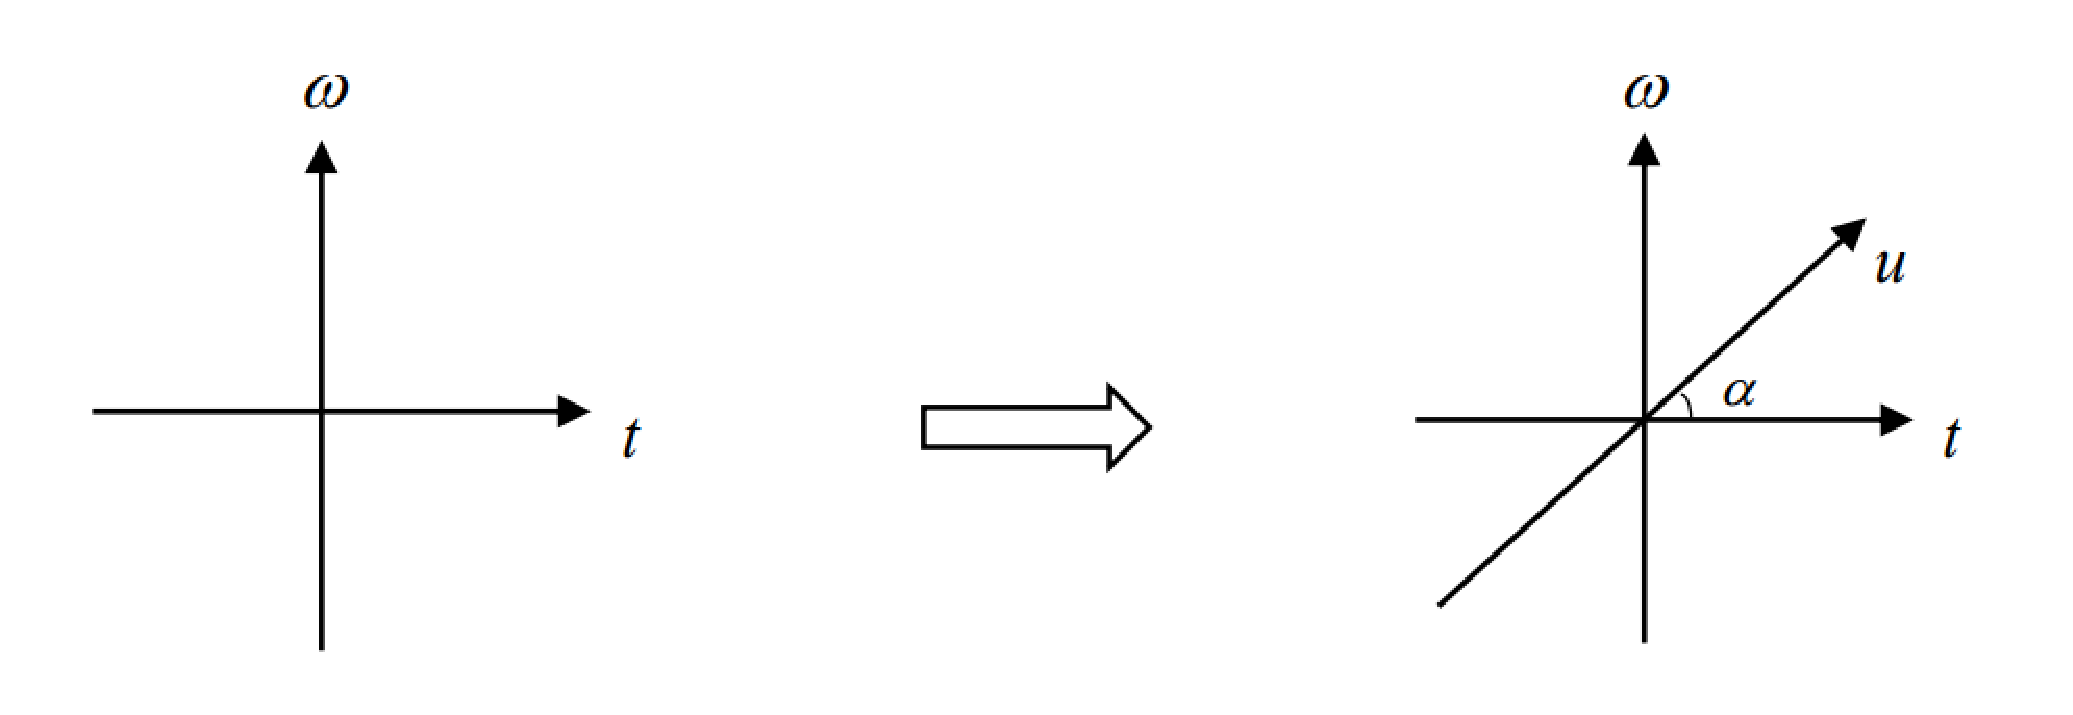
\includegraphics[width = 0.8\textwidth]{figure2_1.eps}
\caption{时频平面旋转示意图}\vspace{-1em}\label{shipinxuanzhuan}
\end{figure}

分数傅里叶变换有着多种定义方式,大致可以分为两大类:经典类分数傅里叶变换(CFRFT)和加权类分数傅里叶变换(WFRFT)。这里仅介绍加权类分数傅里叶变换。

加权分数傅里叶变换是~C.Shih~利用态函数叠加方法提出的一种新的分数傅里叶变换定义。基本思想是利用经典傅里叶变换整数幂运算的~4~周期性,将新的分数傅里叶变换定义成~4~个态函数的线性组合,组合系数则为分数傅里叶变换阶数的函数。对一个信号~$f(x)$~进行~0,1,2,3~次傅里叶变换的结果分别为~$f(x)$~,~$G(x)$~,~$f(-x)$~,~$G(-x)$~,这四个函数便是四项加权分数傅里叶变换(4-WFRFT)的基函数,WFRFT~的定义如下:
\begin{equation}
{\mathcal{F}^\alpha }\left[ {f\left( x \right)} \right] = {\omega _0}\left( \alpha  \right)f\left( x \right) + {\omega _1}\left( \alpha  \right)F\left( x \right) + {\omega _2}\left( \alpha  \right)f\left( { - x} \right) + {\omega _3}\left( \alpha  \right)F\left( { - x} \right)
\end{equation}
其中加权系数${\omega _l}(l = 0,1,2,3)$的定义如下:
\begin{equation}\label{jiaquanxishu}
{\omega _l}(\alpha ) = \cos \left[ {\frac{{(\alpha  - l)\pi }}{4}} \right]\cos \left[ {\frac{{2(\alpha  - l)\pi }}{4}} \right]\exp \left[ {\frac{{3(\alpha  - l)\pi j}}{4}} \right]\;\;\;\;\;(l = 0,1,2,3)
\end{equation}
决定加权系数的变换阶数~$\alpha$~一样以~4~为周期,在~$[0,4]$~区间内变换,图~\ref{xishubianhua}~表明当变换阶数~$\alpha$~变化时,加权系数幅值的变化情况。
\begin{figure}[htbp]
\centering
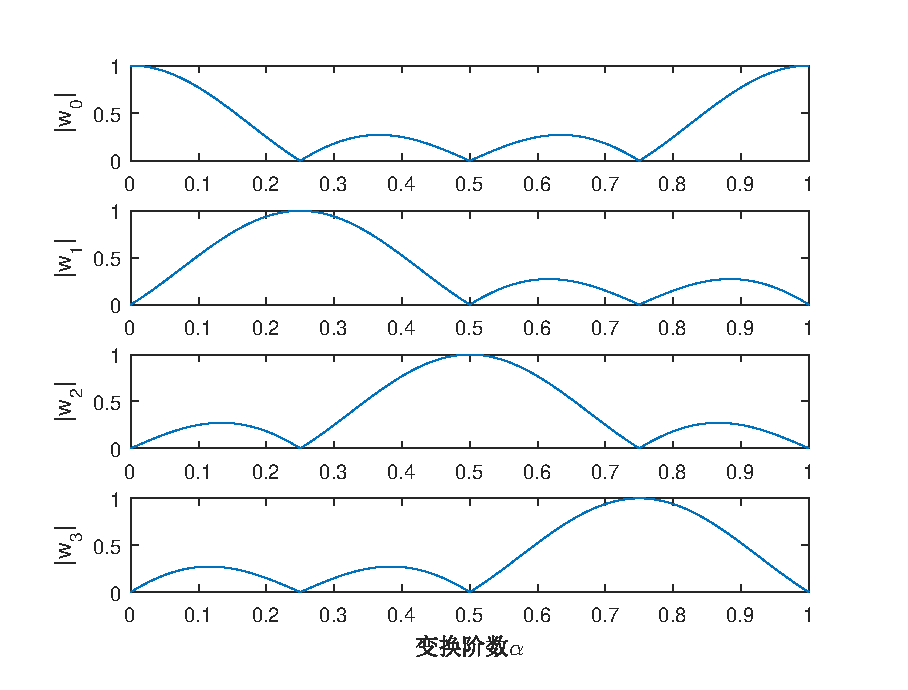
\includegraphics[width = 0.8\textwidth]{figure2_2.eps}
\caption{加权系数的模随变换阶数~$\alpha$~的变化}\vspace{-1em}\label{xishubianhua}
\end{figure}

不难从图中看出随着变换阶数的变化,在~4-WFRFT~后的函数中,原函数与经过傅里叶变换后函数所占比重在发生变化,$\alpha$~逐渐靠近~1~和~3~时,傅里叶变换后函数所占比重在不断增大,$\alpha$~逐渐靠近~0~和~2~时,原函数所占比重在不断增大。

这种加权形式定义的~WFRFT~实现的过程比经典~FRFT~简单,并且也满足一些~FRFT~的性质:
\begin{itemize}
\item 连续性:$\left\{ {{\mathcal{F}^\alpha }:{L^2}\left( R \right) \to {L^2}\left( R \right)} \right\}$~,且~$\alpha$~为连续可变的实数;
\item 边界性:当~$\alpha$~取值为整数时,WFRFT~退变为经典傅里叶变换;
\item 旋转相加性:${\mathcal{F}^\alpha }\left\{ {{\mathcal{F}^\beta }\left[ {f\left( x \right)} \right]} \right\} = {\mathcal{F}^{\alpha  + \beta }}\left[ {f\left( x \right)} \right]$~;
\item 酉性:${\left( {{\mathcal{F}^\alpha }} \right)^{ - 1}} = {\left( {{\mathcal{F}^\alpha }} \right)^H}~$。
\end{itemize}

可以看出,经典~WFRFT~的信号表达形式是一种表达时间与频率的连续函数,然而在实际系统中,这种信号无法产生,因此较大程度限制了其在通信系统中的应用。若想将~WFRFT~应用在通信系统中有必要对其进行离散化,传统离散傅里叶变换~DFT~也同样以~4~为周期,而任意一个具有周期性的算子,均可以通过态函数加权的方式进行分数化,因此这里直接利用~DFT~给出了任意复数序列的~4-WFRFT~。

首先定义一个长度为~$N$~的复数序列~${X_0}$~,${X_1}$~、${X_2}$~、${X_3}$~分别为此序列进行~1~,2~,3~次~DFT~的结果,其能量归一化的~DFT~形式如下
\begin{equation}
\left\{ \begin{array}{l}
{X_1}\left( k \right) = \frac{1}{{\sqrt N }}\sum\limits_{n = 0}^{N - 1} {{X_0}\left( n \right){e^{ - j\frac{{2\pi }}{N}kn}}} \\
{X_0}\left( n \right) = \frac{1}{{\sqrt N }}\sum\limits_{n = 0}^{N - 1} {{X_1}\left( k \right){e^{j\frac{{2\pi }}{N}kn}}}
\end{array} \right.
\end{equation}

参照~WFRFT~的定义公式,序列的离散~WFRFT~定义如下:
\begin{equation}
{S_0} = {\mathcal{F}^\alpha }\left[ {{X_0}} \right] = {\omega _0}\left( \alpha  \right){X_0} + {\omega _1}\left( \alpha  \right){X_1} + {\omega _2}\left( \alpha  \right){X_2} + {\omega _3}\left( \alpha  \right){X_3}
\end{equation}

采用矩阵的形式表示如下
\begin{equation}
  \begin{array}{l}
  {\bf{S}} = \left[ \begin{array}{l}
  {S_0}\\
  {S_1}\\
  {S_2}\\
  {S_3}
  \end{array} \right] = {{\bf{W}}_\alpha }{\bf{X}} = \left[ {\begin{array}{*{20}{c}}
  {{\omega _0}}&{{\omega _1}}&{{\omega _2}}&{{\omega _3}}\\
  {{\omega _3}}&{{\omega _0}}&{{\omega _1}}&{{\omega _2}}\\
  {{\omega _2}}&{{\omega _3}}&{{\omega _0}}&{{\omega _1}}\\
  {{\omega _1}}&{{\omega _2}}&{{\omega _3}}&{{\omega _0}}
  \end{array}} \right]\left[ \begin{array}{l}
  {X_0}\\
  {X_1}\\
  {X_2}\\
  {X_3}
  \end{array} \right]\\
  \;\;\;\;\;\;\;\;\;\;\;\;\;\;\;\;\;\;\;\;\;\; = \left[ {\begin{array}{*{20}{c}}
  {{\omega _0}{X_0} + {\omega _1}{X_1} + {\omega _2}{X_2} + {\omega _3}{X_3}}\\
  {{\omega _3}{X_0} + {\omega _0}{X_1} + {\omega _1}{X_2} + {\omega _2}{X_3}}\\
  {{\omega _2}{X_0} + {\omega _3}{X_1} + {\omega _0}{X_2} + {\omega _1}{X_3}}\\
  {{\omega _1}{X_0} + {\omega _2}{X_1} + {\omega _3}{X_2} + {\omega _0}{X_3}}
  \end{array}} \right]
  \end{array}
\end{equation}
其中,${S_1}$~,${S_2}$~,${S_3}$~分别是序列~${S_0}$~的~1~,2~,3~次~DFT~。可以看出~${S_0}$~,${S_1}$~,${S_2}$~,${S_3}$~分别是~${X_0}$~,${X_1}$~,${X_2}$~,${X_3}$~的~$\alpha$~阶~WFRFT~变换且满足如下关系:
\begin{equation}
{S_3} = \mathcal{F}[{S_2}] = {\mathcal{F}^2}[{S_1}] = {\mathcal{F}^3}[{S_0}]
\end{equation}

通过上面给出的定义形式,可以看出~WFRFT~可以对输入的任意复数序列进行变换并通过相应阶数的逆变换还原原始输入序列。可以直接应用于通信系统中。需要注意的,离散化~WFRFT~的变换结果并不等同于对传统的~WFRFT~进行采样,这点与傅里叶变换与~DFT~的关系不同,原因在于若对经典~WFRFT~采样,其时域和频域的量纲不统一。

%%%%%%%%%%%%%%%%%%%%%%%%%%%%%%%%%%%%%%%%%%%%%%%%%%%%%%%%%%%%%%
\subsection{基于~4-WFRFT~的变换域通信系统}

对于四项加权形式定义的~FRFT~,在计算某一信号的~4-WFRFT~时,由于~4~个加权项的特殊性,实际上就是对信号的时域信息和频域信息进行加权相加,因此它的计算复杂度要小于经典定义类型的~FRFT~,因其是通过~DFT~定义的,在计算中可以直接利用快速傅里叶算法~FFT~计算,计算量与~FFT~相当,也因此更容易在工程中实现。

~4-WFRFT~模块的物理实现过程如图~\ref{jiaquanshixianguocheng}~:
\begin{figure}[htbp]
\centering
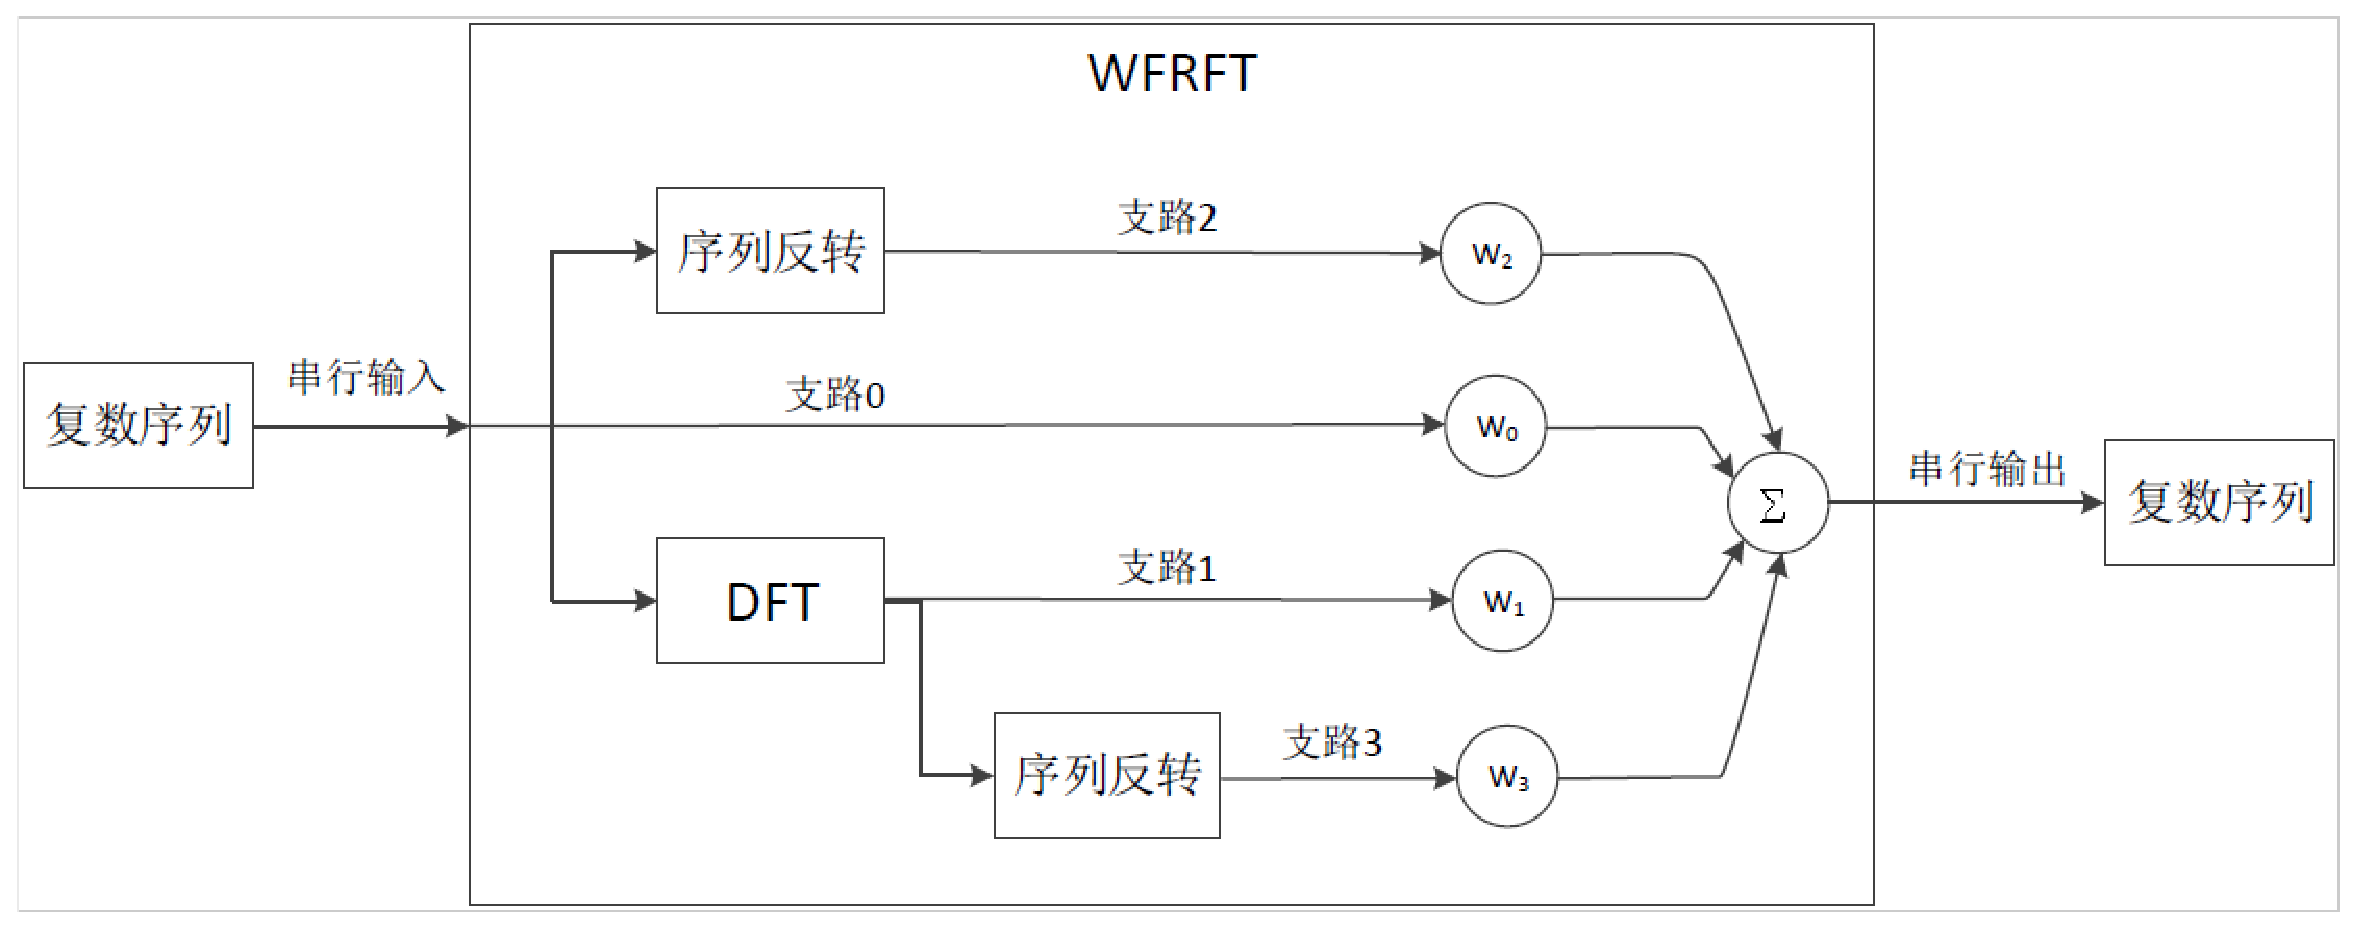
\includegraphics[width = 0.9\textwidth]{figure2_4.eps}
\caption{4-WFRFT~物理实现过程}\vspace{-1em}\label{jiaquanshixianguocheng}
\end{figure}
长度为~$N$~的复数序列~$X_0$~为原始需调制信号,分四路进行加权求和,其中两路为原始时域信号与其反转后的信号,另外两路信号为原始序列经~DFT~的结果与其反转,在实现过程中当~$N$~为~2~的整数次幂时可以直接用~FFT~模块代替~DFT~,即完成一次~4-WFRFT~变换仅需一次~DFT~和两次信号反转,计算量与实际系统中实现的复杂程度与~FFT~相近。容易在通信系统中实现。其变换过程数学模型如下:
\begin{equation}\label{WFRFTgongshi}
\begin{split}
{S_0}(n) = {w_0} \cdot {X_0}(n) + {w_1} \cdot \frac{1}{{\sqrt N }}\sum\limits_{k = 0}^{N - 1} {{X_0}(k){e^{ - j\frac{{2\pi }}{N}kn}}}\\
 +  {w_2} \cdot {X_0}( - n) + {w_3} \cdot \frac{1}{{\sqrt N }}\sum\limits_{k = 0}^{N - 1} {{X_0}(k){e^{j\frac{{2\pi }}{N}kn}}}
\end{split}
\end{equation}

对比~OFDM~系统和单载波频域均衡系统的实现结构不难看出:支路~1~,3~均经过~DFT~处理后进行加权,对应了~OFDM~信号的并行传输过程;而另外两支路没有~DFT~模块仅是一次反转,没有其他处理操作,实际上是简单的单载波串行传输的过程。实际上,由于~4-WFRFT~定义形式的特殊性,对信号进行~4-WFRFT~的过程中的时域频域信息与现有通信系统中对信号进行单载波和多载波调制的表述形式相一致。可以看成~4-WFRFT~是将单载波系统与多载波系统融合起来,实现的混合载波调制。并且~4-WFRFT~输出信号的时频特征与其调制阶数~$\alpha$~有直接关系,改变参数~$\alpha$~可以实现单载波调制与多载波调制之间的转换,使用于现有的通信发射、接受系统,不需要额外开销。WFRFT~通信系统较之于传统通信系统由于加权阶数的引入,可以更加灵活的应对某些特定信道条件,可以通过搜寻最优化的变换阶数~$\alpha$~来使系统整体性能最优化。

基于~WFRFT~在数字通信中的物理意义,文献[]的作者给出了混合载波通信系统模型如图~\ref{xitongjiegou}~:
\begin{figure}[htbp]
\centering
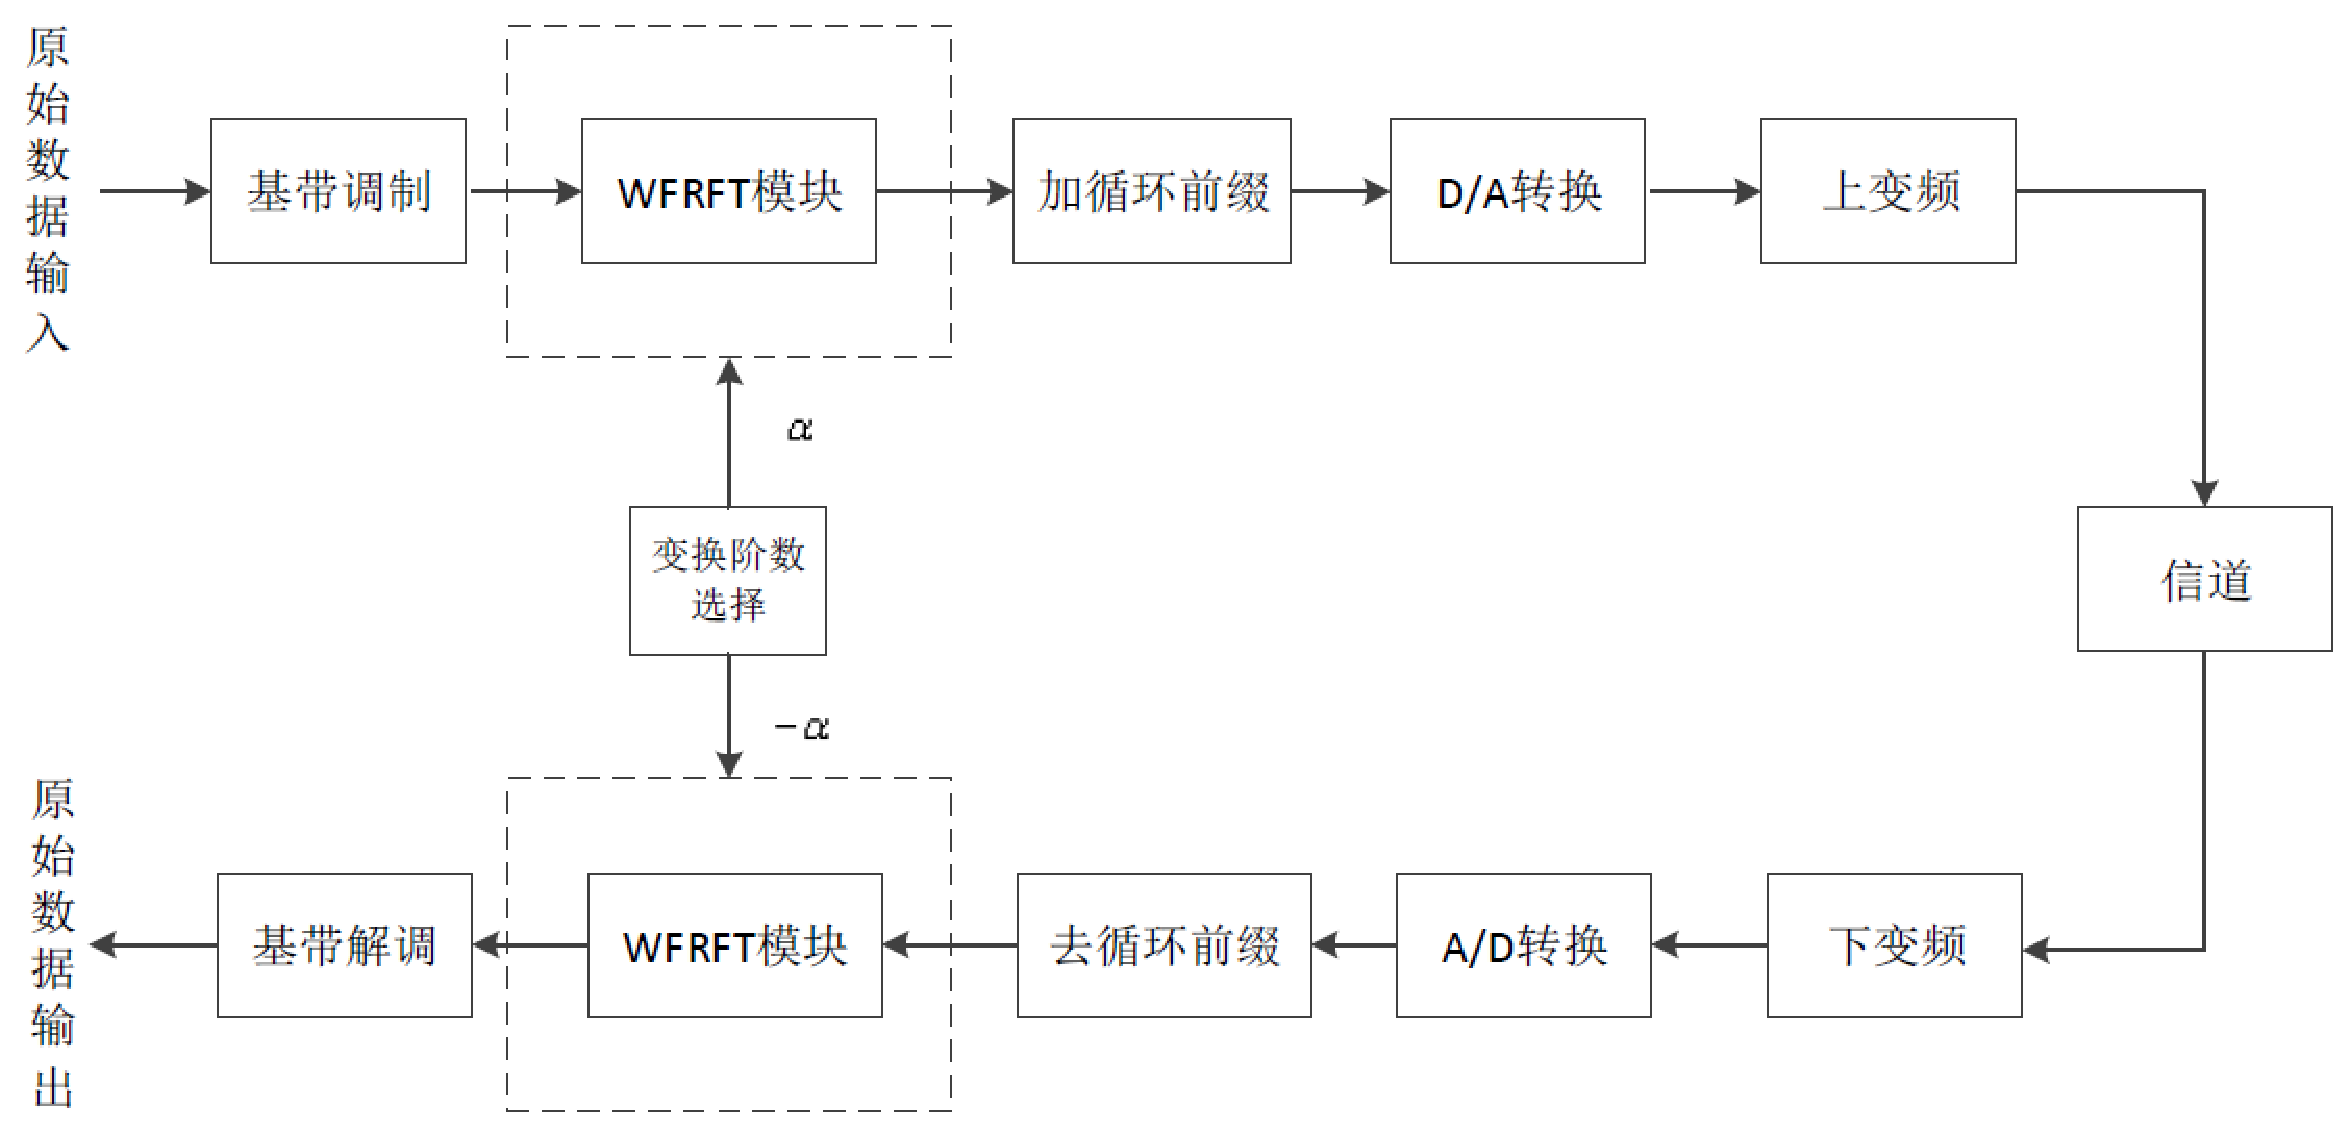
\includegraphics[width = 0.9\textwidth]{figure2_3.eps}
\caption{基于~4-WFRFT~通信系统结构}\vspace{-1em}\label{xitongjiegou}
\end{figure}

从图中可以看出,混合载波通信系统与~OFDM~系统相似,该通信系统模型可以在基于块传输方式的单载波和~OFDM~系统之间实现平滑过渡:通过阶数~$\alpha$~进行转换,当~$\alpha$~为非整数时,系统对应为单载波与多载波的混合形式。这一方面可以作为沟通传统单载波、多载波体制的桥梁;另一方面,在很多复杂、多变的环境或条件约束下,混合载波通信系统可能具有较传统载波体制更灵活的应对方式和更好的性能表现。

从上面的分析得到,~4-WFRFT~对信号的处理过程实际上包含了单载波与多载波的实现过程,所以,~4-WFRFT~变换后的信号特征也与传统调制下的信号有所不同。根据式~(\ref{WFRFTgongshi})~给出的~4-WFRFT~数学表达定义可以看出,~4-WFRFT~的输出信号形式不仅仅与输入信号的信息有关,在很大程度上由加权系数来决定变换后信号中所含时频信息的比重,加权系数又由变换阶数~$\alpha$~决定,当~$\alpha$~变化时引起各个加权信号的幅值伸缩与相位旋转,从而决定了~4-WFRFT~输出信号的不同。图~\ref{xingzuotu}~给出了~QPSK~信号分别经过变换阶数为~0~,0.1~,0.25~,1~的~4-WFRFT~变换处理后的星座图,
\begin{figure}[htbp]
\centering
\subfigure{\label{xingzuo1}}\addtocounter{subfigure}{-2}
\subfigure{\subfigure[~$\alpha$~= 0]{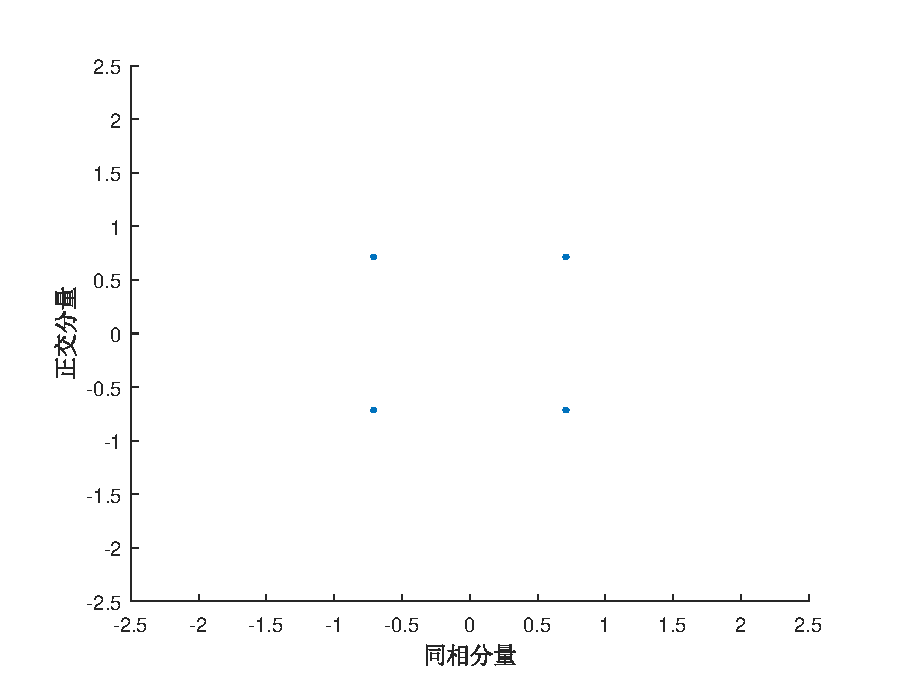
\includegraphics[width=0.4\textwidth]{xingzuo0.eps}}}
\subfigure{\label{xingzuo2}}\addtocounter{subfigure}{-2}
\subfigure{\subfigure[~$\alpha$~= 0.1]{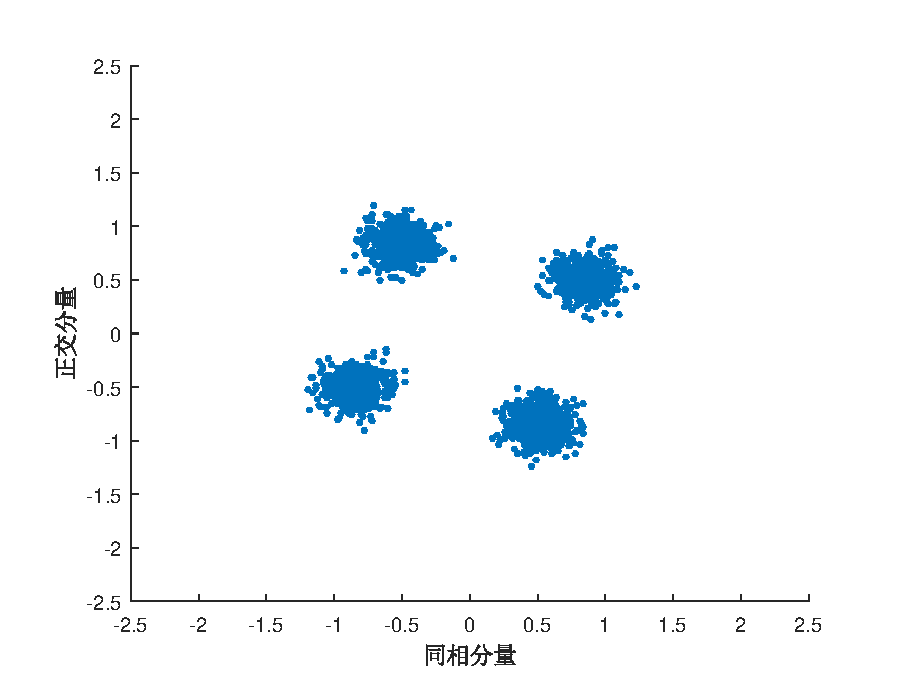
\includegraphics[width=0.4\textwidth]{xingzuo01.eps}}}
\subfigure{\label{xingzuo3}}\addtocounter{subfigure}{-2}
\subfigure{\subfigure[~$\alpha$~= 0.25]{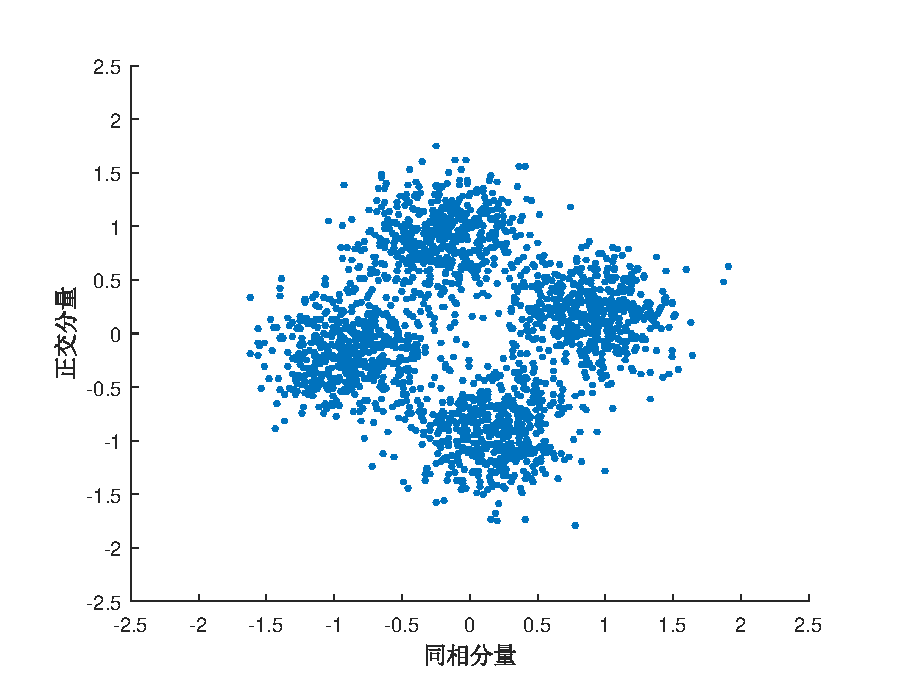
\includegraphics[width=0.4\textwidth]{xingzuo025.eps}}}
\subfigure{\label{xingzuo4}}\addtocounter{subfigure}{-2}
\subfigure{\subfigure[~$\alpha$~= 1]{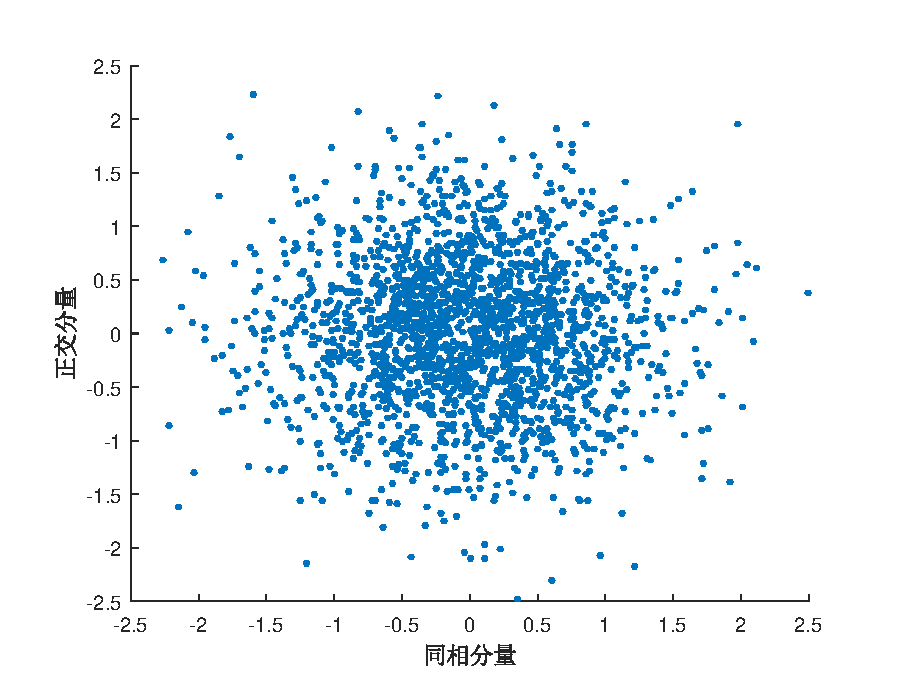
\includegraphics[width=0.4\textwidth]{xingzuo1.eps}}}
\caption{~4-WFRFT~变换后信号星座图}\label{xingzuotu}\vspace{-1em}
\end{figure}
可以看出随着~$\alpha$~的增大,原本重叠在一起的星座点逐渐旋转并散开,随着~$\alpha$~进一步增大,星座点的边界逐渐模糊,信号所含频域成分逐渐增加,最终当~$\alpha$~增大到~1~时,所有信号点完全混叠在一起,无法区分,在复平面呈现出一种类高斯的分布,在接收端只有通过与之对应的~$-\alpha$~阶反变换才能够将信号正确解调。通过信号星座图的描绘,展现了~WFRFT~信号灵活多变的特点。单参数~WFRFT~信号的星座图会随着阶数的改变而呈现发散、 旋转、 汇聚等变化, 星座点分布呈现类高斯特性。WFRFT~的这种信号形式比传统比传统单载波和多载波信号具有更均匀的时频能量分布。这一分布特性有利于信号在复杂多变的场景中,以及时频域同时存在干扰的信道下保持性能鲁棒性。
